\documentclass[a4paper,pdftex]{article}
\usepackage{titlesec}
\usepackage{wrapfig}
\usepackage{fancyvrb}
\usepackage{amsfonts}
\usepackage{palatino}
\usepackage{lastpage}
\usepackage{color}
\usepackage{t1enc}
\usepackage[isolatin]{inputenc}
\usepackage[pdftex]{graphicx}
\usepackage{fancyhdr}
\usepackage{endnotes}
%\usepackage[pdftitle={Der Titel},pdftex=true,bookmarks=true,a4paper=true,
%           colorlinks=true,linkcolor=blue,filecolor=black,pagecolor=black,urlcolor=red, 
%            citecolor=blue]{hyperref}
             
  \lhead{\itshape \subsectionmark}
  \chead{} \rhead{\itshape Page \thepage{} of \pageref{LastPage}}
  \renewcommand{\headrulewidth}{0pt}
  \lfoot{\mbox{}\\ \itshape SnipSnap Developer Guide}
  \cfoot{}
  \rfoot{\mbox{}\\ \itshape  March 2004}
  
  \begin{document}
  
  \thispagestyle{empty}

  %\setcounter{page}{0}  %% Titelseite nicht mitzaehlen
  {\raggedleft\vspace{15cm}{
   \huge\bfseries\sffamily{SnipSnap Developer Guide}\\\vspace{0.5cm}
  \normalsize\itshape Fraunhofer FIRST\\
  February 2004\\\vspace{16cm}}
 
   \fbox{\parbox{\textwidth}{
   \textbf{Contact:} \\
   \begin{tabbing}
   Stephan J. Schmidt\= \quad \qquad \qquad \=
   Matthias L. Jugel \\
   stephan@mud.de \> \>
   leo@mud.de\\
   \end{tabbing}
   }}
   }
 
  \newpage
  \pagestyle{empty}
  \tableofcontents
  \newpage
  \pagestyle{fancy}
  %%\setcounter{page}{1}  %% Titelseite nicht mitzaehlen

\section{Introduction}


\section{SnipSnap CVS access}

While there are source code releases of SnipSnap, which you should normally use,
the latest source code can be accessed through CVS. CVS is a source code revision
control system\cite{CVS}. It's available for nearly all plattforms and already part of Linux and
MacOS X.

\begin{verbatim}
cvs -d :pserver:anonymous@cvs.first.fraunhofer.de:/var/cvs login
Password: press <Return> when asked for a password
cvs -d :pserver:anonymous@cvs.first.fraunhofer.de:/var/cvs checkout snip
\end{verbatim}

\section{Naming conventions}

The naming of classes in SnipSnap follows some conventions, beside the standard naming conventions
in Java.

\begin{itemize}
\item \textit{<Name>Support} is a support class that cannot be used on it's own, most of the time an abstract class. Example FilterSupport
\item \textit{Base<Name>} is a class with basic functionality which can be instantiated. Probably implements the interface <Name>. Example BaseRenderEngine
\item \textit{<Name>Impl} or \textit{Default<Name>} is a class that implements the interface <Name>. Usually this is the only implementation, otherwise it would be named Base<Name>. Example SnipSpaceImpl.
\item \textit{Mock<Name>} is a Mock object that implements <Name> or subclasses <Name>
\end{itemize}

\section{SnipSnap rendering}

SnipSnap uses the Radeox\cite{Radeox} render engine for rendering the text markup to HTML.
Radeox knows macros and filters to do the rendering job. Some macros and filters, like the BoldFilter
are part of Radeox. Others, which are specific to SnipSnap, are part of SnipSnap (Picture \ref{Architecture}).

\begin{figure}[ht]
  \centering
    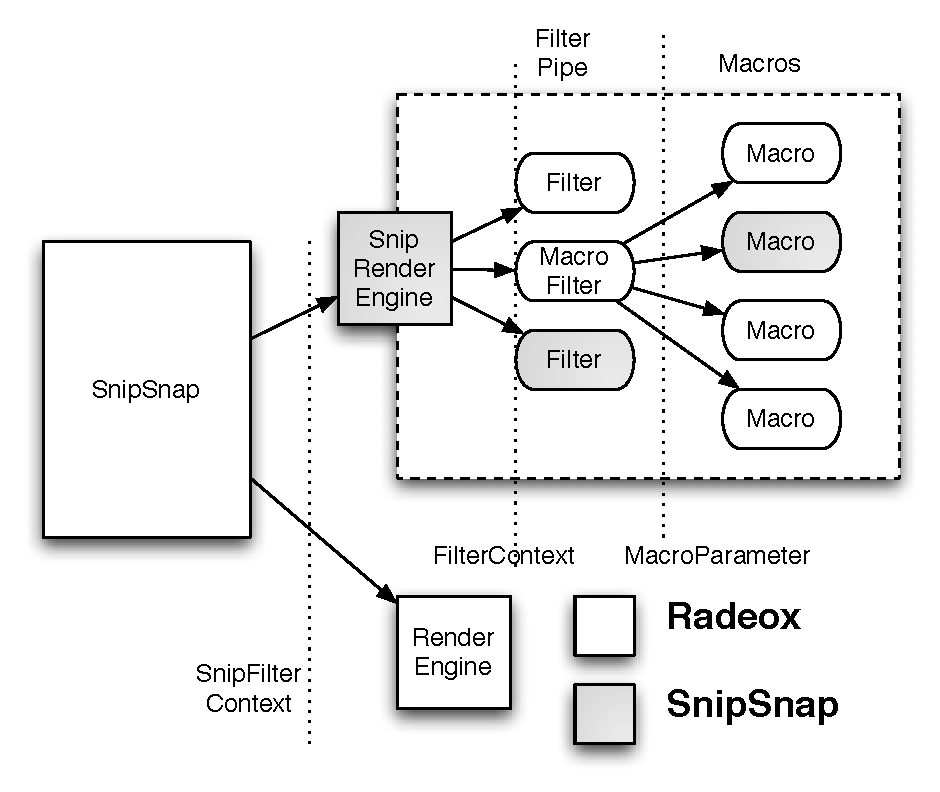
\includegraphics[keepaspectratio,width=8cm]{images/SnipRadeox}
     \caption{\small\textsf Radeox Render Architecture}
     \label{Architecture}
\end{figure}

\subsection{Writing Macros}

For writing  Macros you should take a look at the Radeox Developer Guide. This Guide explains in 
detail how to write Macros. The section here will explain how to write macros that interact with
SnipSnap. Radeox is the render engine behind SnipSnap. But Radeox macros don't know about SnipSnap. 
So it's not possible in Radeox macros to get the current Snip etc. So there are new classes in SnipSnap,
inherited from their Radeox counterparts, which get the information about the SnipSnap context.

\subsubsection{Getting the snip from which the macro is rendered}

Suppose you want to write a macro which displays the snip from which it was rendered.
Instead of inheriting from BaseMacro you inherit your macro from SnipMacro. This
way you get the correct context information from SnipSnap.

%!SRC|examples/HelloSnipMacro.java|start-1|end-1|
\begin{Verbatim}[gobble=0,frame=single,numbers=left,fontsize=\small]
public class HelloSnipMacro extends SnipMacro {

  public void execute(Writer writer, SnipMacroParameter params)
    throws IllegalArgumentException, IOException {

    SnipRenderContext context = params.getSnipRenderContext();
    Snip snip = (Snip) context.getAttribute("snip");
    writer.write("hello, my name is "+snip.getName());
  }


  public String getName() {
    return "hello-snip";
  }
}
\end{Verbatim}
%!END

While Radeox macros get a MacroParameter object, SnipSnap macros get a SnipMacroParameter. From the parameter
you get the current RenderContext, which is of type SnipRenderContext. SnipRenderContext stores several attributes,
one of them is the current snip from which the macro was rendered. The Snip is accessed with the key SnipRenderContext.SNIP.
This might not be the displayed snip. Then you get the name from the snip and write it to the writer as usual.

\subsubsection{Getting access to the component container}

SnipSnap uses a Pico component container\cite{PicoContainer}. If you need
to access some components in SnipSnap like the storage backend or the messaging
component, SnipRenderContext gives you a reference to the container.

%!SRC|examples/MessageSendMacro.java|start-1|end-1|
\begin{Verbatim}[gobble=0,frame=single,numbers=left,fontsize=\small]
public class MessageSendMacro extends SnipMacro {

  public void execute(Writer writer, SnipMacroParameter params)
    throws IllegalArgumentException, IOException {

    SnipRenderContext context = params.getSnipRenderContext();
    Snip snip = (Snip) context.getAttribute("snip");
    PicoContainer container = (PicoContainer)
      context.getAttribute("container");

    MessageService service = (MessageService)
      container.getComponentInstance(MessageService.class);
    Message message = new Message("SNIP_VIEWED",
                                  snip.getName());
    service.send(message);
  }


  public String getName() {
    return "send-message";
  }
}
\end{Verbatim}
%!END

\subsubsection{Getting access to displayed snip}

As mentioned before, the snip from which a macro is rendered might not
be the displayed snip. There are a lot of snip used on one SnipSnap page, 
for example every portlet is a snip. If your macro is called from whithin a
portlet, the displayed snip differes from the snip from which your macro
was called. SnipRenderContext has an attribute for the currently displayed
snip. With this it's easy to write for example a menu macro.

\subsubsection{Getting access to the loggend in user}

If you want to get access to the logged in user, there is an user attribute
in the SnipRenderContext. If you want to write a macro which greets the user,
you first get the user, check if he is logged in, get his name and then write
a greeting.

%!SRC|examples/GreetUserMacro.java|start-1|end-1|
\begin{Verbatim}[gobble=0,frame=single,numbers=left,fontsize=\small]
public class GreetUserMacro extends SnipMacro {

  public void execute(Writer writer, SnipMacroParameter params)
    throws IllegalArgumentException, IOException {

    SnipRenderContext context = params.getSnipRenderContext();
    User user = (User) context.getAttribute("user");
    // Users which are not logged in are guests
    if (user.isGuest()) {
      writer.write("Hello, unknown friend.");
    } else {
      writer.write("Hello, " + user.getLogin());
    }
  }

  public String getName() {
    return "greet";
  }
}
\end{Verbatim}
%!END

User has some other interesting properties, like his last login time, last logout time or
his email adress.

\subsection{Writing Filters}

Filters replace som input with some output. For more information on filters
read the Radeox Developer Guide\cite{RadeoxDeveloper}. As with macros,
filters in SnipSnap are slightly different to give you the context of the filter
call. The FilterContext which is given to filter is of type SnipFilterContext.
After casting you have acces to the SnipRenderContext, which is the same
as for macros.

This example writes over every snip who last modified the snip,
 e.g. \textit{stephan wrote: ...}.

%!SRC|examples/UserFilter.java|start-1|end-1|
\begin{Verbatim}[gobble=0,frame=single,numbers=left,fontsize=\small]
public class UserFilter extends FilterSupport {
  public String filter(String input, FilterContext context) {
    //! Refactor to context like SnipRenderContext
    SnipRenderContext renderContext =
      ((SnipFilterContext) context).getSnipRenderContext();
    Snip snip = (Snip) renderContext.getAttribute("snip");
    return snip.getMUser()+" wrote:\n\n";
  }
}
\end{Verbatim}
%!END

\section{Attachments}

Every snip can store attachments. In the basic implementation, snips are stored
in the file system. You can read, write and manipulate attachments from
e.g your macros. If you want to store attachments with another backend,
you have to implement an AttachmentStorage.

\subsection{Accessing Attachments}

The first example reads all attachments from a snip and then prints them
to a writer.

%!SRC|examples/ShowAttachmentsMacro.java|start-1|end-1|
\begin{Verbatim}[gobble=4,frame=single,numbers=left,fontsize=\small]
    Attachments attachments = snip.getAttachments();
    Iterator iterator = attachments.iterator();
    while (iterator.hasNext()) {
      Attachment attachment = (Attachment) iterator.next();
      writer.write(attachment.getName());
      if (iterator.hasNext()) {
        writer.write(", ");
      }
    }
\end{Verbatim}
%!END

The Attachments object stores a collection of attachments, while the attachment object 
represents a single attachment. Beside the name, each attachment has a size, content type, 
storage date and a physical location.

\subsection{Reading Attachments}

If you need to read an attachment from  the storage for example to display it or store it in another place, you need physical I/O access to the attachment. The attachment I/O is done by the AttachmentStorage component.

%!SRC|examples/AttachmentTest.java|start-1|end-1|
\begin{Verbatim}[gobble=6,frame=single,numbers=left,fontsize=\small]
      Attachments attachments = snip.getAttachments();
      Attachment attachment =
          attachments.getAttachment("MyAttachment.txt");
      AttachmentStorage attachmentStorage = (AttachmentStorage)
          Components.getComponent(AttachmentStorage.class);
      InputStream in = attachmentStorage.getInputStream(attachment);
\end{Verbatim}
%!END

\subsection{Writing Attachments}

Writing Attachments is the same as reading attachment. You first create an attachment object,
then get the OutputStream from the AttachmentStorage and write your attachment data to the
backend.

%!SRC|examples/AttachmentTest.java|start-2|end-2|
\begin{Verbatim}[gobble=6,frame=single,numbers=left,fontsize=\small]
      AttachmentStorage attachmentStorage = (AttachmentStorage)
          Components.getComponent(AttachmentStorage.class);
      OutputStream out =
          attachmentStorage.getOutputStream(attachment);
\end{Verbatim}
%!END

\subsection{Writing an AttachmentStorage}

To change the storage backend for attachment to something you need, e.g. JDBC, WebDAV, CVS or Subversion
you have to implement the AttachmentStorage interface. The I/O methods all throw IOExceptions.

\begin{verbatim}
public interface AttachmentStorage {
  public boolean exists(Attachment attachment);
  public OutputStream getOutputStream(Attachment attachment);
  public InputStream getInputStream(Attachment attachment);
  public void delete(Attachment attachment);
}
\end{verbatim}

For an example we write a MapAttachmentStorage which stores the attachment in memory in a Map object.

%!SRC|examples/MapAttachmentStorage.java|start-1|end-1|
\begin{Verbatim}[gobble=0,frame=single,numbers=left,fontsize=\small]
public class MapAttachmentStorage
    implements AttachmentStorage {

  private Map storage;

  public MapAttachmentStorage() {
    storage = new HashMap();
  }

  public boolean exists(Attachment attachment)
      throws IOException {
    return storage.containsKey(attachment.getLocation());
  }

  public OutputStream getOutputStream(Attachment attachment)
      throws IOException {
    ByteArrayOutputStream out = new ByteArrayOutputStream();
    storage.put(attachment.getLocation(), out);
    return out;
  }

  public InputStream getInputStream(Attachment attachment)
      throws IOException {
    ByteArrayOutputStream out = (ByteArrayOutputStream)
        storage.get(attachment.getLocation());
    byte[] data = out.toByteArray();
    return new ByteArrayInputStream(data);
  }

  public void delete(Attachment attachment) throws IOException {
    storage.remove(attachment.getLocation());

  }
\end{Verbatim}
%!END

\section{Storage Architecture and SnipSpace}

SnipSpace is a facade component to access all snips.

SnipSpace provides
\begin{itemize}
\item fulltext search capabilites
\item persistence for snips
\item a frontend to blogs
\end{itemize}

\begin{figure}[ht]
  \centering
    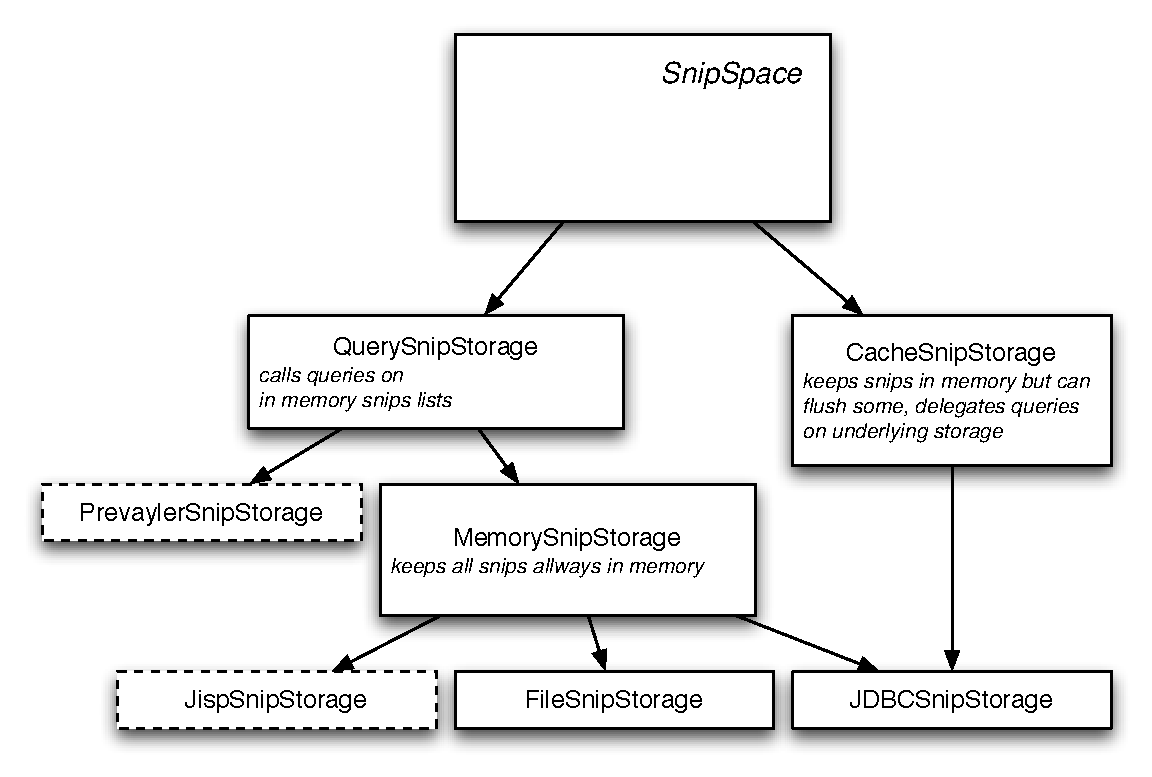
\includegraphics[keepaspectratio,width=8cm]{images/Backend}
     \caption{\small\textsf SnipSnap storage options}
     \label{Backend}
\end{figure}

SnipSpace also handles delayed storage and some statistic information about the 
snips of the space.

\section{Writing a Snip storage backend}

Snips can be stored in different locations. All storage functionality
is encapsulated in SnipStorage components. The SnipStorage component is used
by the SnipSpace component to persist snips. The basic SnipSnap distribution
includes a JDBCSnipStorage, a PropertyFileSnipStorage and a XMLFileSnipStorage.
The JDBC storage stores snips in a JDBC source, the property storage and the XML storage
store snips in the file system. While property storage uses one property file for metadata and
a text file for the snip content, the XML storage persists snips in XML files.

\subsection{FileSnipStorage}

FileSnipStorage is a base class for storing snips in a file system.
You can extend FileSnipStorage but it's recommended to implement
the bases classes for FileSnipStorage in SnipSnap. There are also two bases 
classes for FileStorage

\begin{description}
\item[OneFileSnipStorage]Stores snip in one file
\item[TwoFileSnipStorage]Stores snip in two files
\end{description}

They both handle creation and deletion of files and directories as necessary.
You only need to implement the serialization and deserialization from and to
streams. Both storages also implement the VersionStorage for versioning
information, which usually is stored in sub directories and uses your
persisting methods.

\subsubsection{OneFileSnipStorage}

To write your own file storage with one file, you extend
OneFileStorage and implement the abstract methods:

\begin{Verbatim}[gobble=0,frame=single,numbers=left,fontsize=\small]
protected abstract Map loadSnip(InputStream in)
  throws IOException;
protected abstract String getFileName();
protected abstract void storeSnip(Snip snip, OutputStream out);
\end{Verbatim}

The loadSnip method gets an input stream, reads the snip data from the stream
and creates a new snip. getFileName returns the file name, which could be based
on the snip name. storeSnip gets a snip and an output stream and persists the
snip into that stream. Which format to serialize or deserialize a snip is up to you.
XMLFileSnipStorage is an example of OneFileStorage which stores snip data 
in XML.
 
\subsubsection{TwoFileSnopStorage}

TwoFileSnipStorage is the same as OneFileSnipStorage. The only difference
is that the two file version assumes you want to store the metadata and the
content of a snip in two different files. So each method of OneFileSnipStorage
is duplicated, one for the metadata and one for the content.

\begin{Verbatim}[gobble=0,frame=single,numbers=left,fontsize=\small]
protected abstract Map loadMetadata(InputStream in) 
  throws IOException;
protected abstract String loadContent(InputStream in)
  throws IOException;
protected abstract String getMetadataFileName();
protected abstract String getContentFileName();
protected abstract void storeContent(Snip snip, 
                                     OutputStream out);
protected abstract void storeMetadata(Snip snip, 
                                      OutputStream out);
\end{Verbatim}

\subsubsection{Writing other snip storages}

Writing your own backend for e.g. LDAP storage, you have
to implement the SnipStorage interface. This supplies methods
for storing, loading and querying the storage for snips.

\subsection{Version backend}

Versioning of snips is encapsulated in the VersionStorage component.
The basic SnipSnap distribution can store versioning information
both in files and a JDBC source. JDBC versioning is done in JDBCVersionStorage
while the FileStorages already implement the VersionStorage interface.

\begin{Verbatim}[gobble=0,frame=single,numbers=left,fontsize=\small]
public interface VersionStorage {
  public List getVersionHistory(Snip snip);
  public Snip loadVersion(Snip snip, int version);
  public void storeVersion(Snip snip);
}
\end{Verbatim}

getVersionHistory returns a List of VersionInfo objects for the snip. loadVersion loads the given
version from the backend, while storeVersion stores the newest version.

%\section{Writing a UserManager}

%\section{Writing components}

%\section{Customizing JSP code}

\begin{thebibliography}{}
\bibitem{Radeox} Radeox,  http://radeox.org
\bibitem{RadeoxDeveloper} Radeox Developer Guide, http://radeox.org/space/Developer
\bibitem{CVS} CVS Revision Control System
\bibitem{Groovy} Groovy programming language, http://groovy.codehaus.org
\bibitem{PicoContainer} Component container, http://www.picocontainer.org/
\bibitem{Friedl} Jeffrey E. F. Friedl, Mastering Regular Expressions, ISBN: 0596002890
\end{thebibliography}
\end{document}
